%\VignetteIndexEntry{siggenes Manual}
%\VignetteKeywords{Expression Analysis}
%\VignetteDepends{siggenes}
%\VignettePackage{siggenes}


\documentclass[a4paper]{article}
\usepackage{amsmath,amssymb,pstricks}
\usepackage{graphicx}


%\setlength{\parindent}{0cm} \setlength{\parskip}{18pt}

\renewcommand{\baselinestretch}{1.1}


\usepackage{/home/Holgers/R-2.0.0/share/texmf/Sweave}
\begin{document}
\title{Identifying differentially expressed genes with
\texttt{siggenes}}

\author{Holger Schwender\\  holger.schw@gmx.de}
\date{}

\maketitle

%\setlength{\parskip}{0pt}

\vspace{12pt}

\begin{abstract}
\noindent In this vignette, we show how the functions contained in
the \texttt{R} package \texttt{siggenes} can be used to perform
both the Significance Analysis of Microarrays (SAM) proposed by
Tusher et al.\ (2001) and the Empirical Bayes Analysis of
Microarrays (EBAM) suggested by Efron et al.\ (2001).

\textbf{Version 1.2.0 and following of \texttt{siggenes} contains completely
new written functions for a SAM analysis with new features. Changes to
former versions are summarized on the following pages.}
\end{abstract}
\thispagestyle{empty}

%\setlength{\parskip}{18pt}

\vspace*{48pt} \centerline{\large \bf{PLEASE NOTE}} \vspace*{18pt}
\noindent Since there is a patent pending for the Significance
Analysis of Microarrays (SAM), this package is only free for
non-commercial users. Non-academic users \textbf{MUST} have a
valid license for the full (Excel) version of the SAM software
programmed at Stanford University, see
\texttt{http://www-stat.stanford.edu/$\sim$tibs/ SAM/index.html}.


\newpage

\section*{Changes in Version 1.2.x}

In the following, new features and changes regarding the usage and
the default settings in \texttt{siggenes} 1.2.0 and following are summarized.
All these changes are concerned with the functions for a SAM analysis.
There are \emph{no} changes in the functions for an empirical Bayes
analysis. These functions will be revised in the next months. Now to the
changes in version 1.2.x:

\leftmargini16pt

\begin{itemize}
\item In former versions, one and two class analyses with modified
$t$-statistics (assuming equal group variances) could be performed by
the function \texttt{sam}, and \texttt{sam.wilc} could be used for the same
analyses with Wilcoxon rank statistics. Now \texttt{sam} can be used to perform
\begin{enumerate}
\item[(a)] one and two class analyses with modified $t$-statistics assuming either
equal or unequal group variances
\item[(b)] a multi-class analysis using a modified $F$-statistic
\item[(c)] one and two class analyses with Wilcoxon rank sums
\item[(d)] an analysis of categorical data such as SNP data using Pearson's $\chi^2$-statistic,
\end{enumerate}

where these analyses can also be done by \texttt{sam.dstat} ((a) and (b)), \texttt{sam.wilc}
or \texttt{sam.snp}, respectively. The latter three functions, however, will not be available
in future versions of \texttt{siggenes}.

It is also possible for the user to write her/his own function that computes the expression
scores and other statistics and use this function in \texttt{sam}.

\item The new implementation is faster and less memory-consuming.

\item Since now Welch's $t$-statistic can also be
used, i.e.\ an analysis assuming unequal variances can be done, this test score is used by
default.

\item While in former versions, the median number of falsely called genes was computed
by default, now the mean number is computed by default.

\item The output of \texttt{sam} (and \texttt{sam.dstat}, \texttt{sam.wilc} and \texttt{sam.snp})
is now an object of class SAM. Methods of these class are \texttt{plot}, \texttt{print},
\texttt{summary} and \texttt{identify}.

\item The functions \texttt{sam.plot} and \texttt{sam.delta} are no longer available.
Instead of using \texttt{sam.plot(sam.out,delta)}, one can now obtain the SAM plot by
\texttt{plot(sam.out,delta)} and the information about the significant genes by
\texttt{summary(sam.out,delta)}. Instead of \texttt{sam.delta(sam.out,delta)}, it is
now possible to use \texttt{print(sam.out,delta)}.

\item The required argument \texttt{data} of \texttt{sam} can now also be an exprSet
object (e.g., the output of \texttt{rma}). If \texttt{data} is an exprSet object, the
required argument \texttt{cl} can be specified by the name of one of the columns of
\texttt{pData(data)}.

\item Initial values for $\Delta$ needn't to be specified anymore. They are now calculated
automatically over the range of all possible values of $\Delta$.


\item The group labels are now selected by a procedure that differs from the method used in previous
versions. The expected expression scores $\bar{d}$, the p-values and the number of falsely
called genes will thus differ between this and previous versions, even if the same random seed
was used.

\item It is possible to do complete permutation by setting the number of permutations, \texttt{B},
either to 0 or to an integer larger than the number of all permutations.

\item Instead of using the quantile of the standard deviations of the genes as fudge factor that is optimal following
the criterion of Tusher et al.\ (2001), one can now specify a quantile (e.g., the median) of
the standard deviations that is used as value for the fudge factor. The new implementation of
the computation of the fudge factor is much faster than the old version.

\item In former versions, the fold change was only computed. In the current version, it can
used as filter, i.e.\ genes will be excluded from further analysis if their fold change
is smaller than some threshold. (The computation of the fold change is only available in the
two class case.)

\item Instead of Wilcoxon rank statistics $W$, standardized Wilcoxon rank statistics $W^*$, i.e.\
$W^*=(W-\text{mean}(W))/\text{sd}(W)$ are computed.

\item It is now possible to approximate the null distribution of the Wilcoxon rank statistics
with the standard normal distribution.

\item In former versions, the $\min\{\text{FDR}\}$ was used in the computation of the $q$-value.
Now the original version of the $q$-value in which the $\min\{\text{pFDR}\}$ is also available.

\item Locus links and gene symbols can be added to the table containing the gene-specific
information on the significant genes when information of the chip type is available.

\item It is now possible to obtain an user-specified SAM plot, i.e.\ one can now specify the
title, the labels, the point type, the color of the points, ...

\item In the output of \texttt{summary}, the differentially expressed genes are now
ordered by their "significance," i.e.\ by their absolute expression scores.

\item The function \texttt{identify} makes it possible to identify genes by clicking on the points
in the SAM plot. Information about the specified gene is given and the gene name can be
added to the plot. It is also possible to open the NCBI webpage corresponding to the locus link.
\end{itemize}

\newpage





\section{Introduction}

Both the Significance Analysis of Microarrays (SAM) proposed by
Tusher et al.\ (2001) and the Empirical Bayes Analysis of
Microarrays (EBAM) suggested by Efron et al.\ (2001) can be used
to identify differentially expressed genes and to estimate the
False Discovery Rate (FDR). The \texttt{R} package
\texttt{siggenes} contains functions for both SAM and EBAM
analyses using either a modified $t$ statistic or Wilcoxon rank
statistics. Additionally, it is also possible to perform a SAM analysis
for both multi-class and categorical data. In this vignette, it is described how these
functions can be used. For details on the algorithms
behind these functions, see Schwender et al.\ (2003) and Schwender (2004).

As usual, it is necessary to load the package.


\begin{Schunk}
\begin{Sinput}
> library(siggenes)
\end{Sinput}
\end{Schunk}



In the following, we use the Golub et al.\ (1999) data set as it
is provided by the \texttt{multtest} package to illustrate how the
SAM and the EBAM analyses can be performed.

\begin{Schunk}
\begin{Sinput}
> library(multtest)
> data(golub)
\end{Sinput}
\end{Schunk}


\texttt{data(golub)} consists of a 3,051x38 matrix \texttt{golub}
containing the expression levels of 3,051 genes and 38 samples, a
vector \texttt{golub.cl} containing the class labels of the 38
samples, and a 3,051x3 matrix \texttt{golub.gnames} whose third
column consists of the names of the genes.

\section{Required Arguments: \texttt{data} and \texttt{cl}}

In the first step of each of the SAM and EBAM analyses,
two arguments are required: \texttt{data} and \texttt{cl}. Table \ref{tab:cl}
summarizes how \texttt{cl} can be specified in the different types of analysis.



\begin{table}[!hb]
\vspace*{8pt}
\centering \caption{Possible ways of specifying \texttt{cl} in the
functions for SAM and EBAM analyses.}\label{tab:cl}
\vspace*{8pt}
\begin{tabular}{l c c c c c c}
\hline\hline
&&two class&\multicolumn{2}{c}{two class paired}&&\\[-4pt]
Function&one class&unpaired&\texttt{vector}&\texttt{matrix}&multi-class&\texttt{pdata}\\
\hline
\texttt{sam}&X&X&X&X&X&X\\
\texttt{sam.dstat}&X&X&X&X&X&X\\
\texttt{sam.wilc}&X&X&X&X&--&X\\
\texttt{sam.snp}&--&X&--&--&X&--\\
\texttt{find.a0}&X&X&X&--&--&--\\
\texttt{ebam.wilc}&--&X&X&--&--&--\\ \hline\hline
\vspace*{4pt}
\end{tabular}
\end{table}


The first required argument, \texttt{data}, is the matrix (or the
data frame) containing the gene expression data that should be
analyzed. Each row of this matrix must correspond to a gene, and
each column must correspond to a sample. In SAM analyses with \texttt{sam},
\texttt{sam.dstat} and \texttt{sam.wilc}, \texttt{data}
can also be an \texttt{exprSet} object (e.g., the output of \texttt{rma} or
\texttt{gcrma}).

The second required argument, \texttt{cl}, is the vector of length \texttt{ncol(data)}
containing the class labels of the samples. In a SAM analysis for two
class paired data, \texttt{cl} can also be a matrix. If \texttt{data}
is an \texttt{exprSet} object, \texttt{cl} can also be the name of the column
of \texttt{pData(data)} containing the class labels.

The correct specification of the class labels depends on the type of data that
should be analyzed. On the basis of this specification, the
functions identify the type of data automatically.

\vspace*{18pt}
\noindent \textbf{One class data.} In the one class case, \texttt{cl} is expected to
be a vector of length $n$ containing only 1's, where $n$ denotes the number of
samples but another value than 1 is also accepted. In the latter case,
this value is automatically set to 1. So for $n=10$, the vector \texttt{cl} is given by

\begin{Schunk}
\begin{Sinput}
> n <- 10
> rep(1, 10)
\end{Sinput}
\begin{Soutput}
 [1] 1 1 1 1 1 1 1 1 1 1
\end{Soutput}
\end{Schunk}


\vspace*{18pt} \noindent \textbf{Two class, unpaired data.} In
this case, the functions expect a vector \texttt{cl} consisting
only of 0's and 1's, where all the samples with class label '0'
belong to one group (e.g., the control group), and the samples
with class label '1' belong to the other group (e.g., the
case group). So if, for example, the first \texttt{n1}$=5$ columns of the
data matrix correspond to controls and the next \texttt{n2}$=5$
columns correspond to cases, then the vector \texttt{cl} is given
by

\begin{Schunk}
\begin{Sinput}
> n1 <- n2 <- 5
> rep(c(0, 1), c(n1, n2))
\end{Sinput}
\begin{Soutput}
 [1] 0 0 0 0 0 1 1 1 1 1
\end{Soutput}
\end{Schunk}


The functions also accept other values than 0 and 1. In this case,
the smaller value is automatically set to 0, and the larger value
to 1. So if, e.g., 1 is used as the label for group 1, and 2 for
the label of group 2, then the functions will automatically set the
class label '1' to 0, and the class label '2' to 1.


\vspace*{18pt} \noindent \textbf{Two class, paired data.} Denoting
the number of samples by $n$, we here have $K=n/2$ paired
observations. Each of the $K$ samples belonging to the first group
(e.g., the after treatment group) is labelled by one of the
integers between 1 and $K$, and each of the $K$ samples belonging
to the other group (e.g., the before treatment group) is labelled
by one of the integers between -1 and $-K$, where the sample with
class label '$k$' and the sample with label $'-k'$ build an
observation pair, $k=1,\ldots,K$. So if, e.g., the first $K=5$
columns of the data matrix contain samples from the before
treatment group, and the next $K=5$ columns contain samples from
the after treatment group, where the samples 1 and 6, 2 and 7,
..., respectively, build a pair, then the vector \texttt{cl} is
given by

\begin{Schunk}
\begin{Sinput}
> K <- 5
> c((-1:-5), 1:5)
\end{Sinput}
\begin{Soutput}
 [1] -1 -2 -3 -4 -5  1  2  3  4  5
\end{Soutput}
\end{Schunk}


Another example: If the first column contains the before treatment
measurements of an observation, the second column the after
treatment measurements of the same observation, the third column
the before treatment measurements of the second observations, the
fourth column the after treatment measurements of the second
observation, and so on, then a possible way to generate the vector
\texttt{cl} for $K=5$ paired observations is

\begin{Schunk}
\begin{Sinput}
> K <- 5
> rep(1:K, e = 2) * rep(c(-1, 1), K)
\end{Sinput}
\begin{Soutput}
 [1] -1  1 -2  2 -3  3 -4  4 -5  5
\end{Soutput}
\end{Schunk}


There is another way to specify the class labels in the two class paired
case: They can be specified by a matrix with $n$ rows and two columns. One of
the column should contain -1's and 1's specifying the before and after
treatment samples. The other column should consist of the integers between 1
and $K$ indicating the observation pairs. So if we consider the last example,
\texttt{cl} can also be specified by

\begin{Schunk}
\begin{Sinput}
> K <- 5
> cbind(rep(c(-1, 1), 5), rep(1:5, e = 2))
\end{Sinput}
\begin{Soutput}
      [,1] [,2]
 [1,]   -1    1
 [2,]    1    1
 [3,]   -1    2
 [4,]    1    2
 [5,]   -1    3
 [6,]    1    3
 [7,]   -1    4
 [8,]    1    4
 [9,]   -1    5
[10,]    1    5
\end{Soutput}
\end{Schunk}

While \texttt{cl} must be specify as described above if \texttt{cl} is a vector,
other values will be accepted if \texttt{cl} is a matrix. In the latter case, the
smaller value of the column of \texttt{cl} containing two different values will be
set to -1, and the larger value to 1. The $K$ different values in the other column
are sorted and set to the integers between 1 and $K$.

\vspace*{18pt} \noindent \textbf{Multi-class case.} In this case, \texttt{cl} should
be a vector containing the integers between 1 and $g$, where $g$ is the number of different
classes. Other labels are accepted but will automatically be set to the integers between
1 and $g$.


\section{Significance Analysis of Microarrays}

In this section, we show how the Significance Analysis of
Microarrays (SAM) proposed by Tusher et al.\ (2001) can be applied
to a data set.

As mentioned in the introduction, the Golub et al.\ (1999) data
set provided by the \texttt{multtest} package is used as our example
data set. The matrix \texttt{golub} contains the expression values of the
3,051 genes and the 38 samples, while the vector \texttt{golub.cl}
consists of the class labels that are either 0 and 1. Additionally, the gene names
are provided by the third column of \texttt{golub.gnames}.

A SAM analysis of the Golub et al.\ (1999) data set (i.e.\ a SAM analysis for
two class unpaired data) can be performed by

\begin{Schunk}
\begin{Sinput}
> sam.out <- sam(golub, golub.cl, rand = 123, gene.names = golub.gnames[, 
+     3])
> sam.out
\end{Sinput}
\begin{Soutput}
SAM Analysis for the Two-Class Unpaired Case Assuming Unequal Variances 
 
   Delta  p0   False Called   FDR
1    0.1 0.5 2424.77   2739 0.443
2    0.7 0.5  262.21   1248 0.105
3    1.3 0.5   12.11    507 0.012
4    1.8 0.5    0.74    210 0.002
5    2.4 0.5    0.01     76 0.000
6    3.0 0.5    0.00     15 0.000
7    3.6 0.5    0.00      5 0.000
8    4.1 0.5    0.00      2 0.000
9    4.7 0.5    0.00      2 0.000
10   5.3 0.5    0.00      0 0.000
\end{Soutput}
\end{Schunk}

The argument \texttt{rand} is set to 123 to make the results of \texttt{sam} reproducible.
The same analysis can be done by

\begin{Schunk}
\begin{Sinput}
> sam.dstat(golub, golub.cl, rand = 123)
\end{Sinput}
\begin{Soutput}
SAM Analysis for the Two-Class Unpaired Case Assuming Unequal Variances 
 
   Delta  p0   False Called   FDR
1    0.1 0.5 2424.77   2739 0.443
2    0.7 0.5  262.21   1248 0.105
3    1.3 0.5   12.11    507 0.012
4    1.8 0.5    0.74    210 0.002
5    2.4 0.5    0.01     76 0.000
6    3.0 0.5    0.00     15 0.000
7    3.6 0.5    0.00      5 0.000
8    4.1 0.5    0.00      2 0.000
9    4.7 0.5    0.00      2 0.000
10   5.3 0.5    0.00      0 0.000
\end{Soutput}
\end{Schunk}

A little bit more information about the SAM analysis can be obtained by

\begin{Schunk}
\begin{Sinput}
> summary(sam.out)
\end{Sinput}
\begin{Soutput}
SAM Analysis for the Two-Class Unpaired Case Assuming Unequal Variances 
 
 s0 = 0.0584  (The 0 % quantile of the s values.) 
 
 Number of permutations: 100  

 MEAN number of falsely called genes is computed.

   Delta      p0   False Called     FDR   cutlow   cutup   j2   j1
1    0.1 0.50014 2424.77   2739 0.44276 -0.17693 0.22839 1434 1747
2    0.7 0.50014  262.21   1248 0.10508 -1.26358 1.43791  737 2541
3    1.3 0.50014   12.11    507 0.01195 -2.29908 2.48765  311 2856
4    1.8 0.50014    0.74    210 0.00176 -3.15356 3.31139  134 2976
5    2.4 0.50014    0.01     76 0.00007 -4.15687 4.25941   44 3020
6    3.0 0.50014    0.00     15 0.00000 -5.57692 5.13946    4 3041
7    3.6 0.50014    0.00      5 0.00000     -Inf 5.97085    0 3047
8    4.1 0.50014    0.00      2 0.00000     -Inf 7.96478    0 3050
9    4.7 0.50014    0.00      2 0.00000     -Inf 7.96478    0 3050
10   5.3 0.50014    0.00      0 0.00000     -Inf     Inf    0 3052
\end{Soutput}
\end{Schunk}

The output of \texttt{sam} contains a table of statistics for a set of initial values
of $\Delta$. If other values of $\Delta$, let's say $1.5, 1.6, 1.7, \ldots,
2.4$, are of interest, one can use \texttt{print} or \texttt{summary} to get the number
of significant genes and the estimated FDR for these values of $\Delta$.

\begin{Schunk}
\begin{Sinput}
> print(sam.out, seq(1.5, 2.4, 0.1))
\end{Sinput}
\begin{Soutput}
SAM Analysis for the Two-Class Unpaired Case Assuming Unequal Variances 
 
   Delta  p0 False Called   FDR
1    1.5 0.5  4.48    377 0.006
2    1.6 0.5  2.37    304 0.004
3    1.7 0.5  1.49    262 0.003
4    1.8 0.5  0.74    210 0.002
5    1.9 0.5  0.43    191 0.001
6    2.0 0.5  0.21    155 0.001
7    2.1 0.5  0.12    132 0.000
8    2.2 0.5  0.06    111 0.000
9    2.3 0.5  0.03     98 0.000
10   2.4 0.5  0.01     76 0.000
\end{Soutput}
\end{Schunk}

The function \texttt{plot} can be used to obtain a graphical display of this table

\begin{verbatim}
plot(sam.out,seq(1.5,2.4,.1))
\end{verbatim}


(see Figure \ref{deltaplot}). It can, however, also generate a SAM plot for a specified value of
$\Delta$

\begin{verbatim}
plot(sam.out,2.4)
\end{verbatim}

(see Figure \ref{samplot}). Note the difference in the specification of \texttt{delta}: If \texttt{delta}
is a vector, a Delta plot as shown in Figure \ref{deltaplot} will be plotted. If \texttt{delta} is a value,
a SAM plot will be generated.

\begin{figure}[!ht]
\vspace{18pt} \small
\centerline{
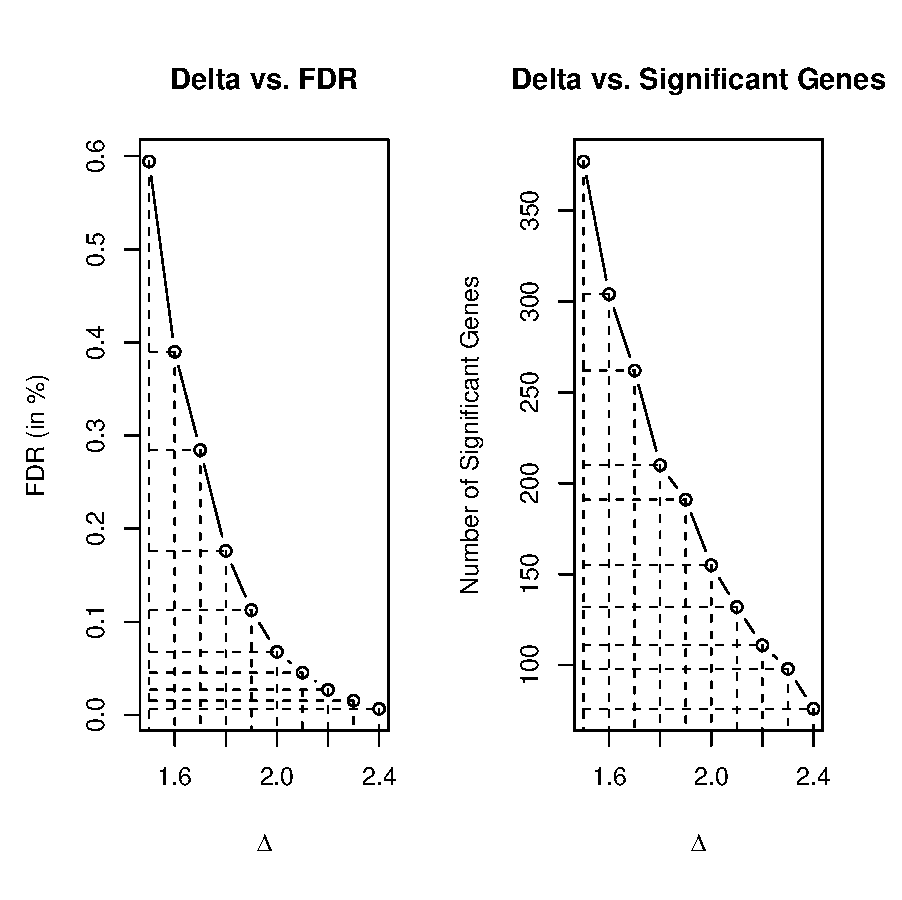
\includegraphics[width=8.5cm]{deltaplot}}\vspace{-15pt}
\caption{Delta plots}\label{deltaplot}

\vspace*{36pt}

\centerline{
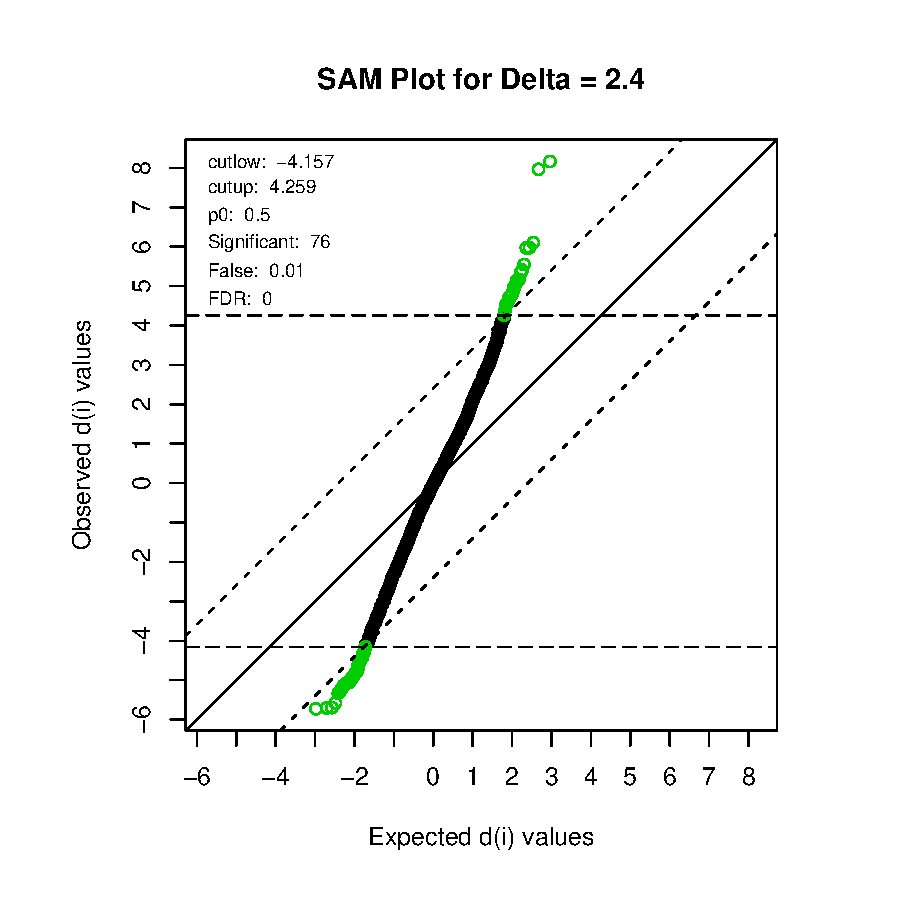
\includegraphics[width=8.5cm]{samplot}}\vspace{-15pt}
\caption{SAM plot for $\Delta=2.4$}\label{samplot}
\vspace*{18pt}
\end{figure}

The function \texttt{identify} makes it possible to obtain information about the genes by
clicking on the SAM plot.

\begin{verbatim}
identify(sam.out,ll=FALSE)
\end{verbatim}

The argument \texttt{ll} is set to \texttt{FALSE} to avoid an error message. If \texttt{chip},
i.e.\ the chip name (e.g., "hgu133plus2"), is specified and \texttt{ll=TRUE}, then the locus link and the
symbol of the gene corresponding to the identified point are added to the output. For example,
clicking on the point nearest to the upper right corner, i.e.\ the point corresponding to the
gene with the largest positive expression score $d$, produces the following output:

\begin{verbatim}
          d.value  stdev p.value q.value R.fold
M27891_at  8.1652 0.2958       0       0 7.2772
\end{verbatim}

If the chip name has been specified either by \texttt{chip} or by setting \texttt{data} to an
\texttt{exprSet} object, one can set \texttt{browse=TRUE} in \texttt{identify}. This opens the NCBI
webpage corresponding to the locus link of the gene identified by clicking on the SAM plot.

Gene-specific information about the genes called differentially expressed using a specific
value of $\Delta$ (here $\Delta=3.3$) can be obtained by

\begin{Schunk}
\begin{Sinput}
> sum.sam.out <- summary(sam.out, 3.3, ll = FALSE)
\end{Sinput}
\begin{Soutput}
SAM Analysis for the Two-Class Unpaired Case Assuming Unequal Variances 
 
s0 = 0.0584  (The 0 % quantile of the s values.) 
 
 Number of permutations: 100  

 MEAN number of falsely called genes is computed.

 Delta: 3.3 
 cutlow: -Inf 
 cutup: 5.97085 
 p0: 0.50014 
 Significant Genes: 5 
 Falsely Called Genes: 0 
 FDR: 0 


Genes called significant:

   Row d.value   stdev p.value q.value  R.fold        Name
1  829 8.16522 0.29583       0       0 7.27718   M27891_at
2 2124 7.96478 0.17787       0       0  3.3953   X95735_at
3 2600 6.10237 0.19112       0       0  2.6687 L09209_s_at
4 2664 5.97575 0.39187       0       0 4.72295 Y00787_s_at
5  766 5.97085 0.17313       0       0 2.49723   M16038_at
\end{Soutput}
\end{Schunk}

The rows of \texttt{golub} that contain the values of the differentially expressed genes
can be obtained by

\begin{Schunk}
\begin{Sinput}
> sum.sam.out$row.sig.genes
\end{Sinput}
\begin{Soutput}
  M16038_at   M27891_at   X95735_at L09209_s_at Y00787_s_at 
        766         829        2124        2600        2664 
\end{Soutput}
\end{Schunk}

the general information about the set of significant genes by

\begin{Schunk}
\begin{Sinput}
> sum.sam.out$mat.fdr
\end{Sinput}
\begin{Soutput}
  Delta        p0 False Called FDR cutlow    cutup j2   j1
1   3.3 0.5001357     0      5   0   -Inf 5.970848  0 3047
\end{Soutput}
\end{Schunk}

and the gene-specific information by

\begin{Schunk}
\begin{Sinput}
> sum.sam.out$mat.sig
\end{Sinput}
\begin{Soutput}
             Row  d.value     stdev p.value q.value   R.fold
M27891_at    829 8.165222 0.2958251       0       0 7.277179
X95735_at   2124 7.964784 0.1778697       0       0 3.395304
L09209_s_at 2600 6.102371 0.1911219       0       0 2.668699
Y00787_s_at 2664 5.975750 0.3918749       0       0 4.722954
M16038_at    766 5.970848 0.1731333       0       0 2.497230
\end{Soutput}
\end{Schunk}

To obtain just the names of the genes called significant using $\Delta=3.3$,

\begin{Schunk}
\begin{Sinput}
> list.siggenes(sam.out, 3.3)
\end{Sinput}
\begin{Soutput}
M27891_at
X95735_at
L09209_s_at
Y00787_s_at
M16038_at
\end{Soutput}
\end{Schunk}

\vspace*{18pt}

\section{Empirical Bayes Analysis of Microarrays}

The original version of the Empirical Bayes Analysis of
Microarrays proposed by Efron et al.\ (2001) is based on the same
modified $t$-statistic also used in SAM. In another paper,
Efron et al.\ (2002) modify this version of EBAM by replacing
the modified $t$ statistic by the Wilcoxon rank sum statistic. In
this section, it is shown how these two versions of EBAM can be
applied to a data set.

\subsection{EBAM with \texttt{find.a0} and \texttt{ebam}}

For their EBAM analysis, Efron et al.\ (2001) summarize the
expression values of each gene by the same modified version of the
usual $t$ statistic that is computed in SAM. The only difference
lies in the computation of the fudge factor. While in the SAM
procedure this computation is automatically done by \texttt{sam},
we here need to specify the fudge factor prior to performing the
main EBAM analysis. Actually, computing the fudge factor $a_0$ for
the EBAM analysis means to perform a (standardized) EBAM analysis
for each specified value of $a_0$, and then selecting the value
that is in some sense optimal. For such a comparison, it is
necessary to always have the same marginal distribution for the
permuted expression scores. For each value of $a_0$, both the
observed and the permuted expression scores are therefore
transformed such that the permuted expression scores follow a
standard normal distribution. This analysis can be performed by

\begin{verbatim}
> find.out <- find.a0(golub, golub.cl, rand = 123)

EBAM Analysis for the two class unpaired case.


 Number of significant genes for some a0:
                 a0=0   a0=0.0606 (alpha=0) a0=0.1148 (alpha=0.1)
                  740                   740                   680
a0=0.1292 (alpha=0.2) a0=0.1428 (alpha=0.3) a0=0.1562 (alpha=0.4)
                  680                   680                   680
a0=0.1695 (alpha=0.5) a0=0.1849 (alpha=0.6) a0=0.2025 (alpha=0.7)
                  649                   649                   649
a0=0.2272 (alpha=0.8) a0=0.2707 (alpha=0.9)
                  623                   623

 Suggested choice for a0: 0
\end{verbatim}

\begin{figure}[!h]
\vspace{18pt} \small \renewcommand{\baselinestretch}{1.2}
\centerline{
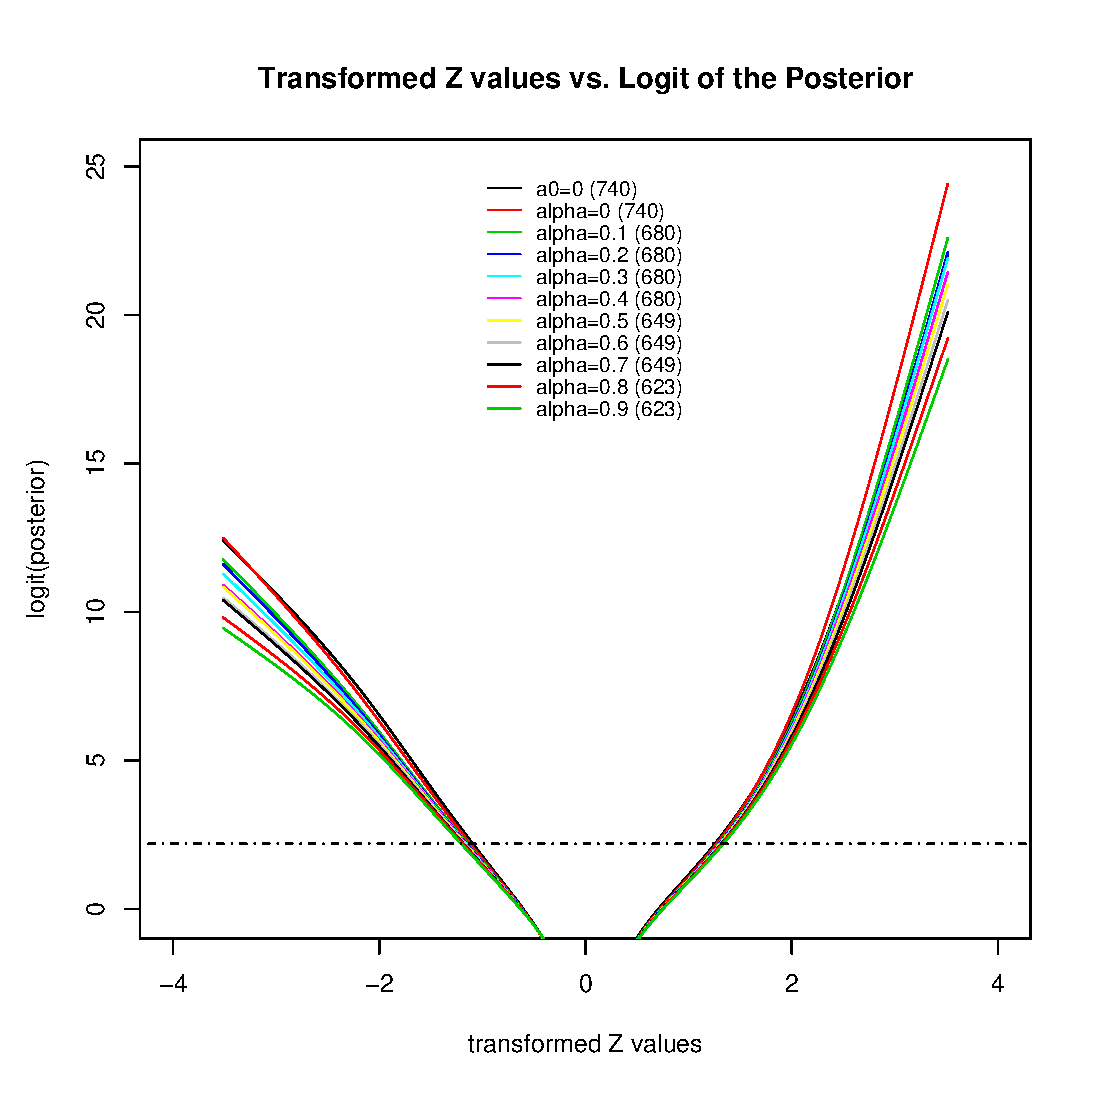
\includegraphics[width=8cm]{logitpost}}\vspace{-12pt}
\caption{Plot of the transformed (observed) expression scores vs.\
the logit of their posterior probabilities.}\label{logitpost}
%\vspace*{18pt}
\end{figure}

The output of \texttt{find.a0} suggests a value for
$a_0$ (here $a_0=0$). This suggestion follows the optimization
criterion of Efron et al. (2001) who argue that the value of $a_0$
should be selected that leads to the most differentially expressed
genes. If there are more than one optimal choice, \texttt{find.a0}
will suggest the smallest of these values.

One, however, should also take a look on the plot of the
transformed observed expression scores vs.\ the logit of their
posterior probabilities (see Figure \ref{logitpost}). If another
value than the suggested value leads to a slightly smaller number
of differentially expressed genes, but has higher posterior
probabilities for the most extreme expression values, then it will
also be appropriate to use this value, since the latter indicates
a better separation between the distribution of all genes and the
distribution of the not differentially expressed genes (cf.\ Efron
et al.\ 2001).



For our analysis with \texttt{ebam}, we use the suggested choice
for $a_0$. Since this value is used as default in
\texttt{ebam}, we do not have to specify \texttt{a0}. Other choices
must be specified. The usage
and the output of \texttt{ebam} is similar to the usage and the
output of \texttt{sam.plot}.

\begin{verbatim}
> ebam.out <- ebam(find.out, gene.names = golub.gnames[, 2])
 Using a0 = 0 and the original Z values, there are
 714 significant genes and 37.75 falsely called genes.
 For p0 = 0.4901 , the FDR is 0.0259 .
\end{verbatim}

\begin{figure}[!ht]
\small \renewcommand{\baselinestretch}{1.2}
\centerline{
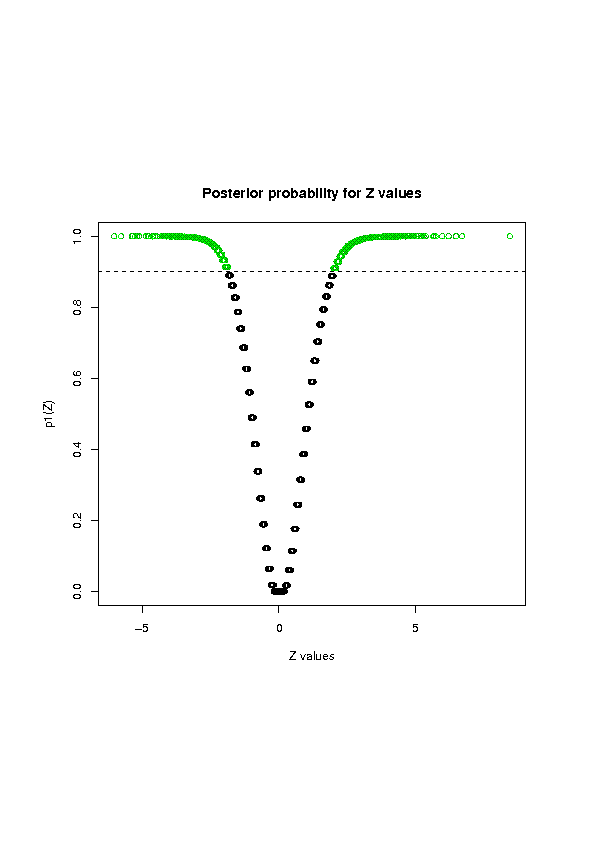
\includegraphics[width=8cm]{ebam}}\vspace{-12pt}
\caption{Plot of the expression scores vs.\ their posterior
probability. Genes called differentially expressed are marked
green.}\label{ebam}\vspace{18pt}
\end{figure}


For each differentially expressed gene, its
expression value $z$, its posterior probability, its $q$-value,
its $R$-fold, and two estimates of its local FDRs (cf.\ Efron et
al. 2001) can be stored in an output file by specifying \texttt{file}. Furthermore,
\texttt{ebam} generates the plot of the posterior probabilities of
the genes in which the differentially expressed genes are marked
green (see Figure \ref{ebam}). The number of genes called differentially
expressed may differ between \texttt{find.a0} and \texttt{ebam}
since in the former the transformed and in the latter the original
expression scores are used. The rows of the data matrix containing
the differentially expressed genes can -- similar to
\texttt{sam.plot} -- be obtained by \texttt{ebam.out\$row.sig.genes}.

\subsection{EBAM with \texttt{ebam.wilc}}

Contrary to the other three analyses, only one function, namely
\texttt{ebam.wilc}, has to be called for the EBAM analysis using
Wilcoxon rank sums (for details of this procedure, see Efron et
al.\ 2002).

\begin{verbatim}
> ebam.wilc.out <- ebam.wilc(golub, golub.cl,rand = 123,
+  g = golub.gnames[, 2])

EBAM-Wilc Analysis for the two class unpaired case.

tied Wilcoxon scores: 5

p0: 0.5078
Number of significant genes: 711
falsely called genes: 37.57
 FDR: 0.0268
\end{verbatim}

Again gene-specific statistics of the differentially expressed
genes and general information on, e.g., the number of
differentially expressed genes and the estimated FDR will be
stored in a file, if \texttt{file} is specified. The general
information are also displayed by \texttt{ebam.wilc} in the
\texttt{R} console. Furthermore, \texttt{ebam.wilc} displays the
number of genes having a tied Wilcoxon rank sum. The expression
score of each of these genes is by default randomly assigned
either to the next larger or smaller integer. Not displayed are
the two plots generated by \texttt{ebam.wilc}. In this plot the posterior
probabilities of the genes are shown and the differentially expressed genes are marked
green.

%\vspace{1cm}

\begin{thebibliography}{}
\item[Efron, B.,] Tibshirani, R., Storey, J.\ D., and Tusher, V.\ (2001),
``Empirical Bayes Analysis of a Microarray Experiment,"
\textit{Journal of the American Statistical Association}, 96,
1151--1160.

\item[Efron, B.,] and Tibshirani, R.\ (2002), ``Empirical Bayes Methods
and False Discovery Rates for Microarrays," \textit{Genetic
Epidemiology}, 23, 70--86.

\item[Golub, T.\ R.,] Slonim, D.\ K., Tamayo, P., Huard, C., Gaasenbeek,
M., Mesirov, J.\ P., Coller, H., Loh, M.\ L., Downing, J.\ R.,
Caliguiri, M.\ A., Bloomfield, C.\ D., and Lander, E.\ S.\ (1999),
``Molecular Classification of Cancer: Class Discovery and Class
Prediction by Gene Expression Moni\-to\-ring," \textit{Science},
286, 531--537.

\item[Schwender, H.,] Krause, A., and Ickstadt, K.\ (2003), ''Comparison of
the Empirical Bayes and the Significance Analysis of Microarrays,"
\textit{Techical Report}, University of Dortmund, Dortmund, Germany,
\texttt{http://www.sfb475.uni-dortmund.de/berichte/tr44-03.pdf}.

\item[Schwender, H.] (2004), ''Modifying Microarray Analysis Methods for
Categorical Data -- SAM and PAM for SNPs." To appear in: \emph{Proceedings
of the the 28th Annual Conference of the GfKl}.

\item[Tusher, V.\ G.,] Tibshirani, R., and Chu, G.\ (2001),
``Significance Analysis of Microarrays Applied to the Ionizing
Radiation Response," \textit{Proceedings of the National Academy
of Science,} 98, 5116--5121.

\end{thebibliography}



\end{document}
